% !TeX encoding = UTF-8
% !TeX spellcheck = en_US
% !TeX root = main.tex

\documentclass[12pt,a4paper]{memoir}
\usepackage[utf8]{inputenc}
\usepackage{amsmath}
\usepackage{amsfonts}
\usepackage{amssymb}
\usepackage{graphicx}
\usepackage{rotating}
\usepackage{epstopdf}
\usepackage{hyperref}
%\usepackage{indentfirst}
\usepackage[english]{babel}
\usepackage{empheq}

\usepackage[colorinlistoftodos,textsize=scriptsize]{todonotes}

% Default fixed font does  support bold face

% Custom colors
\usepackage{color}
\definecolor{deepblue}{rgb}{0,0,0.5}
\definecolor{deepred}{rgb}{0.6,0,0}
\definecolor{deepgreen}{rgb}{0,0.5,0}
\definecolor{gray}{rgb}{0.5,0.5,0.4}

\usepackage{listings}
\usepackage{lstautogobble}
\renewcommand{\lstlistingname}{Code example}

% Python style for highlighting
\newcommand\pythonstyle{\lstset{
    language=Python,
    basicstyle=\linespread{1}\footnotesize\ttfamily,
    otherkeywords={self},             % Add keywords here
    keywordstyle=\footnotesize\ttfamily\bfseries\color{deepblue},
    emph={MyClass,__init__},          % Custom highlighting
    emphstyle=\bf\color{deepred},    % Custom highlighting style
    stringstyle=\color{deepgreen},
    frame=tb,                         % Any extra options here
    showstringspaces=false,           % 
    tabsize=4,
    numbers=left,    
    numberstyle=\tiny\color{gray}, 
    breaklines=true,
    autogobble=true,
    commentstyle=\color{gray},           
}}


% Python environment
\lstnewenvironment{python}[1][]
{
\pythonstyle
\lstset{#1}
}
{}

% Python for external files
\newcommand\pythonexternal[2][]{{
\pythonstyle
\lstinputlisting[#1]{#2}}}

\newcommand\cppstyle{\lstset{
    language=C++,
    basicstyle=\ttfamily,
    keywordstyle=\color{deepblue}\ttfamily,
    stringstyle=\color{red}\ttfamily,
    commentstyle=\color{grey}\ttfamily,
    morecomment=[l][\color{magenta}]{\#},
    autogobble=true,
}}

% C++ environment
\lstnewenvironment{c++}[1][]
{
    \cppstyle
    \lstset{#1}
}
{}

% % % % % % % % % % % % % % % % % %
% trick not to release comments   %
  \newif\ifrelease
%	                              %
	%\releasetrue
	\releasefalse
%	                              %
	\ifrelease
		\renewcommand{\todo}[1]{}
	\fi
% end of trick                    %
% % % % % % % % % % % % % % % % % %

\renewcommand{\vec}[1]{\underline{#1}}
\newcommand{\mat}[1]{\underline{\underline{#1}}}
\newcommand{\scal}[2]{\langle #1 {\,,\,} #2 \rangle}

\newcommand{\remark}{\paragraph{Remark ---}}
\renewcommand{\epsilon}{\varepsilon}
\setsecnumdepth{subsection}
%\maxtocdepth{subsection}

\def\thetitle{Localisation and correction of orbit perturbations in BESSY II storage ring}
\def\thesubject{Master Thesis}
\def\theauthor{Olivier Churlaud}
\author{\theauthor}
\title{\thetitle}

\hypersetup{
    unicode=true,
    pdftitle={\thetitle},
    pdfauthor={\theauthor},
    pdfsubject={\thesubject},
    colorlinks=true,       % false: boxed links; true: colored links
    linkcolor=black,       % color of internal links (change box color with linkbordercolor)
    citecolor=green,
    filecolor=red,
    urlcolor=blue
}

\begin{document}
\frontmatter
\clearpage
\thispagestyle{empty}
\maketitle
\
\vfill
\begin{abstract}
       ......
\end{abstract}
\vfill

\cleardoublepage

\tableofcontents
\listoffigures

\mainmatter
\section{Background}
\label{sec:background}
\subsection{BESSY II}

\todo[inline]{Short history of BESSY II + some numbers = 1/2 page}
\subsection{Storage ring}
\todo[inline]{Purpose + Physics of the accelerator = 3-5 pages}
\subsection{Orbit and distortions}
\todo[inline]{Physics + examples = 1/2 - 1 pges}

% !TeX encoding = UTF-8
% !TeX spellcheck = en_US
% !TeX root = main.tex

\chapter{Orbit correction}
\label{sec:correction}
\section{Some documented methods}

Several global corrections methods are well documented in the literature. The most common ones are the best corrector method and the response matrix method (see Sections~\ref{sec:most_effective_corr}) and \ref{sec:response_matrix}). 

Local orbit bumps (presented in Section~\ref{sec:orbit_bump}) allow local correction and are used to change the path of the orbit (during the injection time for example).

\subsection{Local orbit bumps}
\label{sec:orbit_bump}
\todo[inline]{see Wille p127 and p286}

\subsection{Most effective corrector method}
\label{sec:most_effective_corr}
This method is based on the fact that orbit shifts are often caused by strong localized disturbances. Its goal is to correct particularly each disturbance.

\subsubsection{Principle}

Given a distorted orbit, the optimal gain for each corrector is calculated by a mean square error algorithm (see Eq.~\eqref{eq:gain_bestcorr}, \cite{book:wille}). The corrector which provides the best correction is selected: it is the most effective corrector.

Let's assume that the $i$th corrector, at position $s_i$, has the optical parameters $\beta_i$, $\alpha_i$ and $\Psi_i$, and that $m$ monitors are set around the orbit with parameters $\beta_j$, $\alpha_j$ and $\Psi_j$, and read a displacement $u_j$ from the reference orbit ($1 \leq j \leq m$).

The strength $\kappa_i$ of the field at the position $s_i$ is obtained minimizing the function
\todo{Explain in chap 1.3}
\begin{equation}
    \label{eq:gain_bestcorr}
    f_i(\kappa_i) = \sum\limits_{j=1}^{m} (u_j-x_{ij}(\kappa_i))^2 
                  = \sum\limits_{j=1}^{m} (u_j- \kappa_i h_{ij})^2
\end{equation}

with, if $\Delta \Psi_{ij} := \Psi_j-\Psi_i$,

\begin{align}
    \label{eq:hij}
    x_{ij}(\kappa_i) &= \kappa_i h_{ij} \nonumber\\
                     &= \kappa_i \frac{\sqrt{\beta_i \beta_j}}{2}
                         \left[
                             \frac{\cos(\Delta \Psi_{ij}) - 2\alpha_i \sin(\Delta\Psi_{ij})}
                                  {\tan (\pi Q)} + \sin (\Delta\Psi_{ij})
                         \right].
\end{align}

It follows that 
\begin{equation}
    \kappa_i = \frac{\sum\limits_{j=1}^m u_j h_{ij}}{\sum\limits_{j=1}^m h_{ij}^2}
\end{equation}

The $i$th corrector is attributed the gain $-\kappa_i$ to compensate the field.

\subsubsection{Iterative version}
When the most effective corrector is found, the process is reiterated on the corrected orbit with the remaining correctors. 

By doing this until all corrector are used (or that adding a correction does not improve the orbit) a comprehensive correction is reached.

\subsubsection{Practical issue}
The problem of this method is that each corrector must be tested once, and this for each iteration: the initialization of the correction is long and is then fixed.

Moreover, the correction is less efficient than the other ones presented here~\cite{book:wille}.

\subsection{Response matrix}
\label{sec:response_matrix}

This section is mainly based on~\cite{book:wille}, \cite{art:decker-1991} and \cite{art:plouviez-1999}.

The response matrix $\mat{S}$ is defined by the equation $\vec{X} = \mat{S}\, \vec{\Theta}$ where $\vec{\Theta}$ is the \emph{kick vector} and $\vec{X}$ the vector of \emph{orbit change}. If the accelerator has $M$ monitors and $N$ correctors, $\mat{S}$ is a $M \times N$ matrix.

Every coefficient $\mat{S}_{ij}$ is the orbit change at the position $s_i$ (of the $i$th monitor), for a kick of unity 1 at the position $s_j$ (of the $j$th corrector).

This matrix can be theoretically calculated by using the accelerator model and physics: $\mat{S}_{ij} = h_{ij}$ with the formula in \eqref{eq:hij}. However, the actual storage ring is never exactly the same as the designed one, because of several inaccuracies in its building. A more common way of constructing the response matrix is empirical: each measure cycle, a corrector is given a unitary value and the monitor are read, providing a column of the response matrix.

To do the correction, the inverse problem must be solved. We know the orbit change that we need to obtain a cleaner orbit, using the inverse of the response matrix will provide the correction to apply. Since it's very common to have more monitors than correctors, the matrix is not square. A \emph{singular value decomposition} (SVD) is used on the matrix to provide a pseudo-inversion.

Using the SVD also allows to use only the most significant singular values in the correction.\todo{why do we want this?}

\section{State of the art at BESSY II}

\subsection{The correction}
BESSY II currently uses a Fast Orbit Feedback (FOFB) which is based on a PID correction (proportional response with gain P, integral response with gain I and derivative response with gain D) and the response matrix inversion. The full process goes as presented in Fig.~\ref{fig:block_correction}.

\begin{figure}[!h]
    \centering
    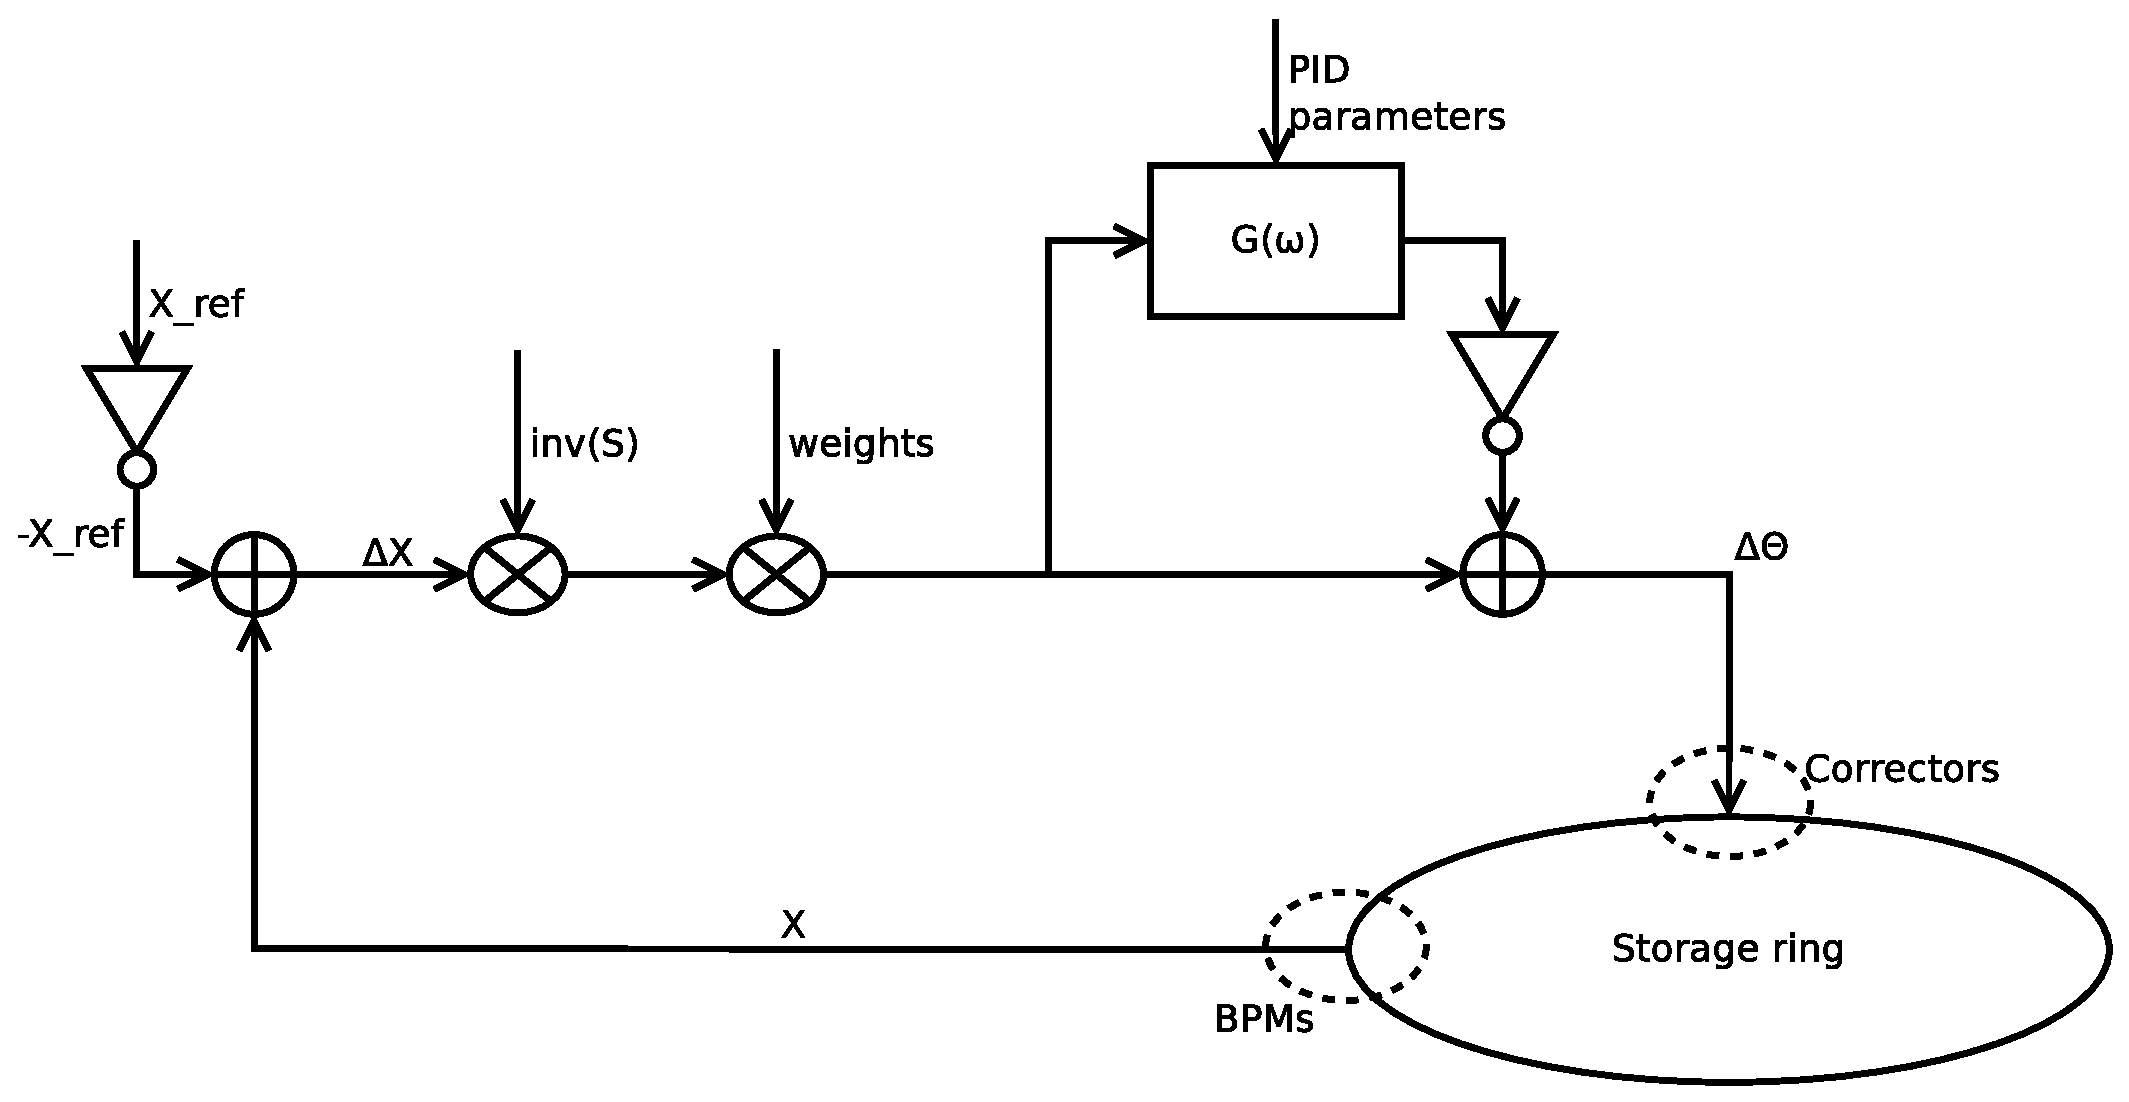
\includegraphics[width=.85\linewidth]{img/correction}
    \caption{\label{fig:block_correction}The correction process}
\end{figure}

\todo[inline]{Should I explain this here with words as well? \newline
    is it $\Delta \Theta$ or $\Theta$ (The real corrector value or the change to add)?\newline
    Why do we need this PID \textbf{\textit{exactly}}?}

\begin{align}
   & \Delta \vec{X} := \vec{X}-\vec{X}_\text{ref} \nonumber \\
   & \Delta \vec{\Theta}_t :=  \mat{S}^{-1} \Delta \vec{X} \odot \vec{W} \nonumber\\
   & G(\omega) = P + \frac{I}{\omega} + D \omega \qquad \text{(the PID)}\nonumber \\
   & \Delta \vec{\Theta} = \left[1-G(\omega)\right] (\Delta \vec{\Theta}_t)
\end{align}
with $\odot$ the point-wise multiplication and, $\vec{W}$ the vector of weights.

\remark The PID gains is not exactly as presented here: to prevent a too violent correction that might destabilize the current in the ring, the proportional gain is increased every correction round by 1\% until it reaches its nominal value.

\remark The PID is implemented as (for the $n$th correction round): 
\begin{equation*}
    P \times \Delta \vec{\Theta}_t(n) + I \times \sum\limits_{k=0}^{n-1}\Delta \vec{\Theta}_t(k) + D \times \left[\Delta \vec{\Theta}_t(n) - \Delta \vec{\Theta}_t(n-1)\right]
\end{equation*}

\subsection{Technical overview}

The correction is naturally automatized. Because the read/write actions should be really fast, a specific infrastructure was designed. This is represented on Fig.~\ref{fig:cbox_mbox}. 

\begin{figure}[!h]
    \centering
    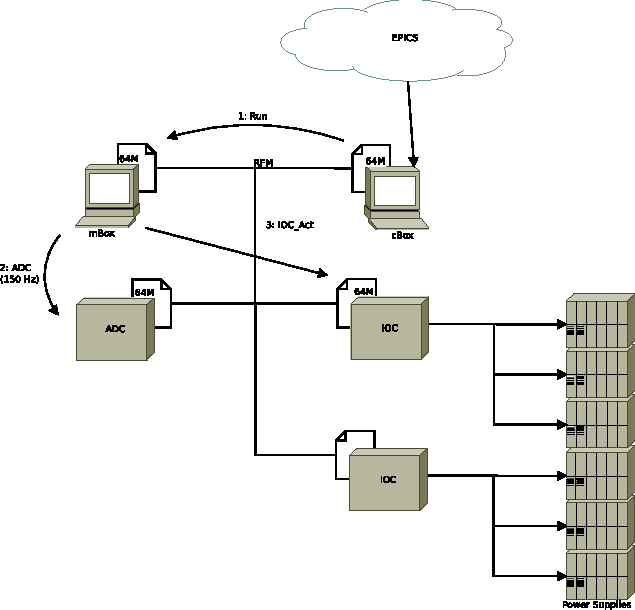
\includegraphics[width=.85\linewidth]{img/mBox_cBox}
    \caption{\label{fig:cbox_mbox}cBox and mBox: the correction infrastructure in BESSY II}
\end{figure}

All elements are connected to a reflective memory (RFM), which provides a high speed and low latency interface. This memory space is split in specified divisions to prevent data collisions.

Two main processes are operating:
\begin{itemize}
    \item the \textbf{cBox}. It controls (= \textit{c}) the correction. It defines when to read the values of the BPMs and when to write the new correction values, it provides initializations values. The operators are communicating with this process to configure the correction.
    \item the \textbf{mBox}. It does the math (= \textit{m}) of the correction. When allowed by the cBox, it reads the BPMs values, do the maths to define the new correction values and write them to the communication bus. This process also publish the values it reads and write so that client programs can subscribe to this data stream and reuse the values internally.
\end{itemize}

After having received the command to run from the cBox, the mBox queries the ADC (Analog-to-Digital Converter) to provide the BPM values in the RFM. The correction is then calculated (in Amperes) and the values are converted in a format easily transmissible. This data is written back to RFM and read by the IOCs (Input-Output Controllers) that relay to the power supplies alimenting the corrector magnets.

The full process is repeated at a frequency of 150~Hz. 

\section{Acquisition of the transfer matrix}

% !TeX encoding = UTF-8
% !TeX spellcheck = en_US
% !TeX root = main.tex

\chapter{Localization of orbit distortion}
\label{sec:localisation}

Correcting the orbit is costly and has never a perfect result. Instead of dealing with the effects, we can deal with the sources of the distortions. If none is really obvious (\textit{eg.} a non-isolated transformer, the 50~Hz perturbation of the main power), the orbit can give us some hints.

We call kick the place where the orbit brutally changes its angle as shown in Fig.~\ref{fig:kick}.

\begin{figure}[!h]
	\centering
	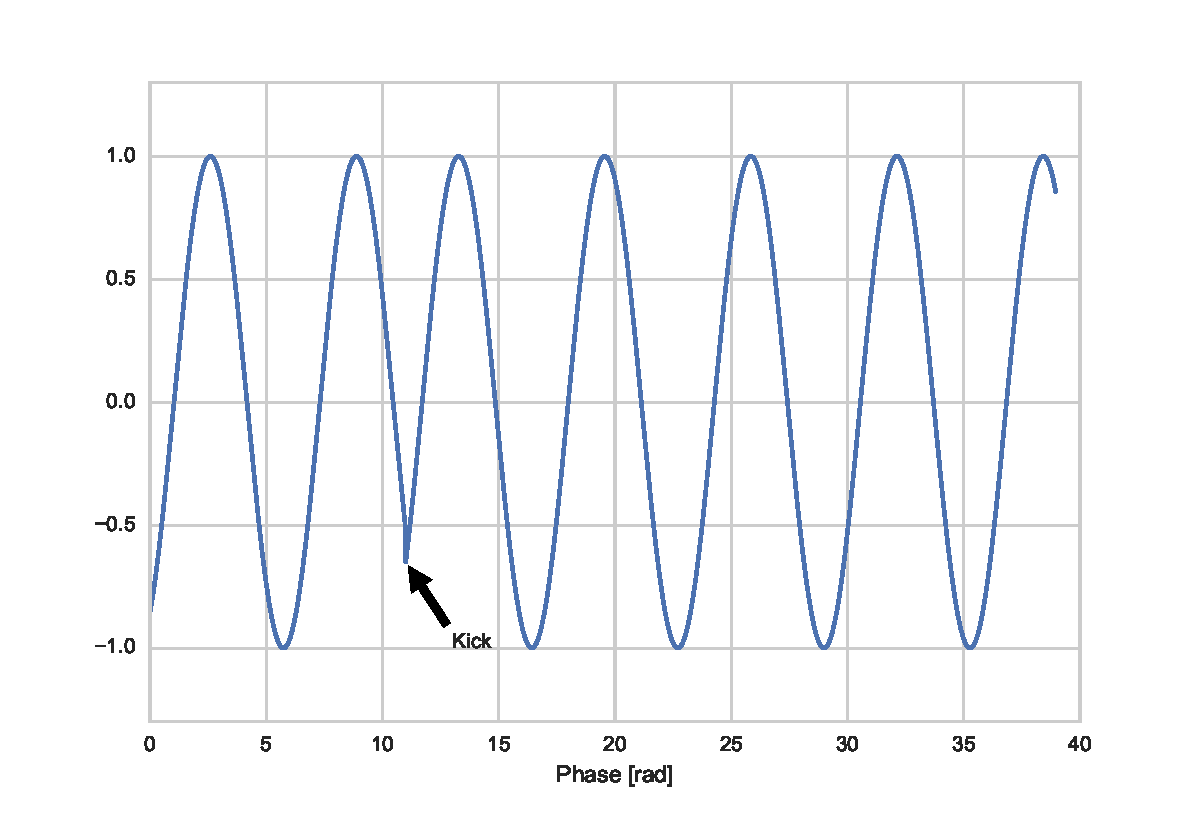
\includegraphics[width=.9\linewidth]{img/kick}
	\caption{\label{fig:kick}Example of kick in the orbit}
\end{figure}

\section{Theory}
\label{ssec:loc_theory}

\subsection{Theoretical setting of the problem}

Everything is described here with the phase variable $\phi = \int\limits_{0}^s \frac{d\sigma}{\beta(\sigma)}$. The spatial variable is only used to have a connection between the result and the actual ring. The explanation will be led with the $x$ variable, but is also valid with the $y$ one.

Let one kick be at $\phi = \hat{\phi}$. The orbit is modified and oscillates with a constant period of $2 \pi$. Because there is {\em only one} kick and according to the closed orbit condition, the oscillation after the kick will be stable for one revolution. Furthermore, the orbit must be continuous on all points, thus at the kick position too.

Let's consider two revolutions, in order to be sure to find one full revolution without kick. Let $\phi_\mathrm{ext} \in [0, 4 \pi Q]$ be this new phase (\textit{ext} for extended). The phase $\phi_0$ where the kick happens is the one so that 
\begin{equation}
\exists (b, c) \in \mathbb{R}^2:
\forall \phi \in [\phi_0, \phi_0 + 2 \pi Q], \quad
x(\phi) = b \sin(\phi + c)
\end{equation}

We have a problem with 3 unknowns to determine: $\phi_0, b, c$. 

\subsection{Practical setting}

We have $m$ BPMs only, distributed around the orbit.
Therefore we define:
\begin{align}
\begin{cases}
\vec{\phi} = [\phi_0, \phi_1, ..., \phi_{m-1}] \\
\vec{x} = [x_0, x_1, ..., x_{m-1}]
\end{cases} \quad \mathrm{and} \quad
\begin{cases}
\vec{\phi}_\mathrm{ext} = [\vec{\phi}, \vec{\phi}+2\pi Q ]\\
\vec{x}_\mathrm{ext} = [\vec{x}, \vec{x}]
\end{cases}
\end{align}

\subsection{Solving the problem}

To find the kick in the orbit it suffices to find a sine that fits in $\vec{x}_\mathrm{ext}$.

An algorithm is designed to find a sine over a revolution, beginning at each BPM and keep the one that fit at best:
\begin{align}
\forall k \in &[0, m-1], \nonumber \\
&\begin{cases}
\vec{\phi}^k = [\vec{\phi}_\mathrm{ext}(k), \vec{\phi}_\mathrm{ext}(k+1), \cdots,  \vec{\phi}_\mathrm{ext}(k+m-1)]\\
\vec{x}^k = [\vec{x}_\mathrm{ext}(k), \vec{x}_\mathrm{ext}(k+1), \cdots,  \vec{x}_\mathrm{ext}(k+m-1)]\\
\tilde{\vec{x}} = \mathtt{fit\_sine}(\vec{x}^k, \vec{\phi}^k)
\end{cases}
\end{align}

It is then defined

\begin{equation}
k_0 = \underset{k \in [0, m-1]}{\textrm{argmin}}\{||\tilde{\vec{x}}-\vec{x}^k||_2\}
\end{equation}

The kick is between $\phi_{k_0-1}$ and $\phi_{k_0+1}$, and we assume that the closest sine is $\tilde{x}(\phi) = b \sin(\phi + c) $.

To find the exact position of the kick, we use the property of closed orbit: the orbit must be continuous also at the kick phase, which means that $\hat{\phi}$ is the solution of
\begin{equation}
b \sin(\phi + c) = b\sin(\phi+c-2 \pi Q), \qquad \mathrm{with}~ \phi \in [\phi_{k_0-1}, \phi_{k_0+1}]
\end{equation}
or, with the numerical approach, 
\begin{equation}
\hat{\phi} =  \underset{\phi \in [\phi_{k_0-1}, \phi_{k_0+1}]}{\textrm{argmin}}\{|b \sin(\phi + c) - b\sin(\phi+c-2 \pi Q)|\}
\end{equation}

\remark For this last step, we use a \textit{linspace} between $\phi_{k_0-1}$ and $\phi_{k_0+1}$ with more than 1000 points.

\remark One should be careful if $k_0 = 0$ (resp. $k_0 = m-1$) and set $\phi_{k_0-1} =\phi_{m-1}$ (resp. $\phi_{k_0+1} = \phi_{0}$). 

\subsection{Finding the good sine}
Several methods are possible to find the best matching sine, for example by using:
\begin{itemize}
	\item a pseudo-inversion
	\item a scalar-product with a sine (resp. a cosine)
\end{itemize}

\paragraph{Pseudo-inversion}
The problem can be set as a linear equation problem as follow.
\begin{align}
&\forall k \in [0,m-1], \tilde{x}(\phi_k) = a_1 \cos(\phi_k) + a_2 \sin(\phi_k) + a \nonumber \\
%
\implies &
\begin{pmatrix}
1 & \cos(\phi_0) & \sin(\phi_0) \\
1 & \cos(\phi_1) & \sin(\phi_1) \\
\vdots & \vdots & \vdots \\
1 & \cos(\phi_{m-1}) & \sin(\phi_{m-1}) \\
\end{pmatrix}
\begin{pmatrix}
a \\ a_1 \\ a_2
\end{pmatrix}
=
\begin{pmatrix}
x_0 \\ x_2 \\ \vdots \\ x_{m-1}
\end{pmatrix} \nonumber
\\
%
\implies &
\begin{pmatrix}
a \\ a_1 \\ a_2
\end{pmatrix}
= 
\mathrm{pseudo\_inv}
\begin{pmatrix}
1 & \cos(\phi_0) & \sin(\phi_0) \\
1 & \cos(\phi_1) & \sin(\phi_1) \\
\vdots & \vdots & \vdots \\
1 & \cos(\phi_{m-1}) & \sin(\phi_{m-1}) \\
\end{pmatrix}
\begin{pmatrix}
x_0 \\ x_2 \\ \vdots \\ x_{m-1}
\end{pmatrix}
\end{align}

The pseudo inverse is calculated in \texttt{Matlab} with \verb$a = M\x$ and in \texttt{python} with \verb$a = numpy.linalg.lstsq(M, x)$ (least-squares solution).

\paragraph{Scalar product with a sine (resp. cosine)}
Since the orbit is expected to be written as
\begin{equation*}
x(\phi) = a_1 \cos(\phi) + a_2 \sin(\phi) + a
\end{equation*}
we can also describe it as
\begin{equation}
x(\phi) = \scal{x}{\cos} \cos(\phi) + \scal{x}{\sin} \sin(\phi) + \scal{x}{1}
\end{equation}
with $\scal{f}{g}$ being the scalar product for real functions: $\int_T f(t)g(u)dt$.

In our numerical case, we approximate this scalar product by its vectorial counterpart by:

\begin{align*}
\scal{\vec{f}}{\vec{g}}: \quad
 &\mathcal{R}^n \times \mathcal{R}^n \longrightarrow \mathcal{R} \\
 & (\vec{f},\vec{g}) \quad\longmapsto \quad \frac{1}{n}\sum\limits_{k=0}^{n-1} f_i g_i
\end{align*}

\paragraph{Coefficient format}
By defining $b = \sqrt{a_1^2+a_2^2}$ and $c = \mathrm{atan2}(a_1, a_2)$  we can write

\begin{equation*}
\tilde{x}(\phi) = a + a_1 \cos(\phi) + a_2 \sin(\phi) = a + b \sin(\phi + c).
\end{equation*} 

\section{Applications}
\todo[inline]{NOT UPDATED: DO NOT CORRECT THIS}
\subsection{Getting the position of a perturbation at a given frequency}
In this section, we deal with a perturbation at a given frequency $f$. The training data is the time signal of all BPMs.

As the perturbation has a known frequency, we extract its complex amplitude from the signal of each BPM with a Fourier transform:

\begin{equation}
\forall i \in [1, \mathrm{BPM\_nb}], \qquad 
\begin{cases}
\vec{X}_i = \mathrm{FFT}(\vec{x}_i) \\
c_i = \vec{X}_i(f)
\end{cases}
\end{equation}

\paragraph{Case of a unique perturbation source}

If the perturbation is unique, then all complex amplitude exactly describe the same sine of frequency $f$ and phase $\alpha_0$. It allows us to describe the complex vector $\vec{c}$ with $\vec{\hat{c}}$, which is real.

\begin{align}
&\alpha_0 = \underset{\alpha \in [0, 2\pi]}{\textrm{argmin}}\{\mathcal{R}e (\vec{c} \cdot e^{-j\alpha}) \} \\
&\vec{\hat{c}} = \mathcal{I}m (\vec{c} \cdot e^{-j\alpha_0})
\end{align}

The new signal $\vec{\hat{c}}$ can be used as an orbit signal: we have one orbit amplitude for each BPM: the kick can be extracted from it with the previous method described in Section \ref{ssec:loc_theory}.


\paragraph{Case of several perturbation sources}
If there are several perturbation sources, a $\alpha_0$ that let the cosine part vanish cannot be found. 


\section{Implementation}
\begin{python}[caption=Get the kick]
	import matplotlib.plt as plt
	import search_kick.core as skcore
	
	# Dataset
	orbit = ..
	phase = ..
	tune = ..
	
	# Get the kick and rebuild the ideal sine
	kick_phase, sin_coef = skcore.get_kick(orbit, phase, tune)
	sine, phase_th = skcore.build_sine(kick_phase, tune, sin_coef)
	
	# Plot the results
	plt.plot(phase, orbit, '-b')
	plt.plot(phase_th, sine, '-g')
	plt.axvline(kick, -2, 2)	
\end{python}


\section{Examples}


\chapter{Harmonic perturbations}
\label{sec:harmonic_distorsion}
\section{Data analysis}

\section{Correction}
\section{Example: the 10 Hz perturbation}

\begin{python}[caption={Perturbation localisation, f = 10 Hz}]
	import matplotlib.plt as plt
	import search_kick.core as skcore
	import search_kick.tools as sktools
	
	# Dataset
	phase = ...
	tune = ...
	time_signal = ....  # nb_bpms lines, nb_samples colunms
	fs = 500  # sampling rate (Hz)
	
	f = 10  # frequency to extract (Hz)
	
	# Extract cosine and sine amplitude with a FFT transform
	a, b = skcore.extract_cos_sin_withfft(values, fs, f)
	
	# Optimize to only have the sine amplitude
	step_size = 0.1
	a_opt, b_opt, alpha_0 = sktools.maths.optimize_rotation(a, b, step_size)
	
	# Get the kick
	kick, sin_coef = skcore.get_kick(a_opt, phase, tune)
	sine, phase_th = skcore.build_sine(kick_phase, tune, sin_coef)
	
	# Plot the results
	plt.plot(phase, a_opt, '-b')
	plt.plot(phase, b_opt, '-m')  # cosine amplitudes: to be sure that it was a unique perturbation
	plt.plot(phase_th, sine, '-g')
	plt.axvline(kick, -2, 2)
	
\end{python}

\chapter{Physics of particle accelerators -- Definitions}
This section is mostly based on~\cite{book:wille}.

\subsection{Notations}
\begin{itemize}
	\item The frame of reference is $K = (\mathbf{x},\mathbf{y},\mathbf{s})$ which origin follow the beam, $\mathbf{x}$ being the horizontal axis (directed toward the exterior of the orbit and normal its the curve), $\mathbf{y}$ being the vertical axis, and $\mathbf{s}$ the tangential axis of the orbit.
	\item $x'(s) = \frac{dx}{ds}$
\end{itemize}

\subsection{Parameters ===== Still wrong.. read again}
\begin{itemize}
	\item $s$ = position in in the orbit (in m)
	\item $Q$ = tune (cf 3.207)
	\begin{equation}
		Q = \frac{\Delta \Psi}{2 \pi}= \frac{1}{2 \pi} \oint \frac{ds}{\beta(s)}
	\end{equation}
	
	\item $\phi(s)$ = phase (in rad)  (cf 3.216)
	\begin{equation}
		\phi(s) = \frac{1}{Q} \int\limits_{0}^s \frac{d\sigma}{\beta(\sigma)} \qquad \in [0, 2 \pi Q]
	\end{equation}
	
	\item $x(s)$ = transverse oscillation of the orbit (cf 3.206) 
	\begin{equation}
		x(s) = \sqrt{\epsilon}\sqrt{\beta(s)}\cos[\Psi(s)+\phi(s)]
	\end{equation}
\end{itemize}
\subsubsection{Condition to fulfill}
\begin{itemize}
	\item Closed orbit: the orbit is circularly continuous in all points. Especially:
	\begin{equation}
	\begin{cases}
	x(\phi = 0) = x(\phi = 2 \pi Q) \\
	y(\phi = 0) = y(\phi = 2 \pi Q)
	\end{cases}
	\end{equation}
\end{itemize}

KLT~\cite{book:wang_2012}
%%
%  Bibliography
%%
\bibliographystyle{IEEEtran}
\bibliography{biblio.bib}

\end{document}

